%%%%%%%%%%%%%%%%%%%%%%%%%%%%%%%%%%%%%%%%%%%%%%%%%%%%%%%%%%%
%%% PLEASE COMPILE WITH XELATEX TO GET THE FONT SIZES RIGHT
%%%%%%%%%%%%%%%%%%%%%%%%%%%%%%%%%%%%%%%%%%%%%%%%%%%%%%%%%%%
\documentclass[11pt,a4paper]{article}
\usepackage[xetex]{geometry}
\usepackage[utf8]{inputenc}
\usepackage{xcolor}
\usepackage{parskip}
\usepackage{mathtools}
\usepackage{physics}
\usepackage[xetex]{hyperref}
\usepackage{hypertoc}
\usepackage{enumitem}
\usepackage{mathspec} % Use no explicit math shapes (CMU is used)
\usepackage{titlesec,titletoc}
\usepackage[singlelinecheck=false]{caption}
\usepackage{tikz}

\geometry{top=1in,bottom=1in,left=1in,right=1.375in}

\setmathfont(Latin){Minion Pro}
\setmathrm{Minion Pro}
\setmathsf{Myriad Pro Light}
\exchangeforms{phi}
\defaultfontfeatures{
	Ligatures={Required,Common,Contextual,Rare,Historic,TeX},
%	Style=Swash,
	Contextuals={Swash,WordInitial,WordFinal}
}
\setmainfont{Minion Pro}
[
	UprightFeatures={
		SizeFeatures={
			{Size={-8.4},Font=* Caption},
			{Size={8.4-13},Font=*},
			{Size={13-19.9},Font=* Subhead},
			{Size={19.9-},Font=* Display}
		},
	},
	BoldFeatures={
		SizeFeatures={ 
			{Size={-8.4},Font=* Bold Caption},
			{Size={8.4-13},Font=* Bold},
			{Size={13-19.9},Font=* Bold Subhead},
			{Size={19.9-},Font=* Bold Display}
		},
	},
	ItalicFeatures={
		SizeFeatures={ 
			{Size={-8.4},Font=* Italic Caption},
			{Size={8.4-13},Font=* Italic},
			{Size={13-19.9},Font=* Italic Subhead},
			{Size={19.9-},Font=* Italic Display}
		},
	},
	BoldItalicFeatures={
		SizeFeatures={ 
			{Size={-8.4},Font=* Bold Italic Caption},
			{Size={8.4-13},Font=* Bold Italic},
			{Size={13-19.9},Font=* Bold Italic Subhead},
			{Size={19.9-},Font=* Bold Italic Display}
		},
	},
]
\setsansfont{Myriad Pro}
\newfontfamily\headlinefont{Myriad Pro Light}

%\linespread{1.3} % Only touch if the linespacing is insufficient

\definecolor{niceBlue2}{RGB}{16,117,175}
\colorlet{activeColor}{niceBlue2}
\hypersetup{
	colorlinks=true,
	linkcolor=activeColor,
	urlcolor=activeColor,
	citecolor=activeColor,
}\urlstyle{same}

\titleformat{\section}[hang]
	{\headlinefont\LARGE}
	{\thesection}
	{12pt}
	{\color{activeColor}}
\titlespacing{\section}{0em}{4ex}{1ex}
\titleformat{\subsection}[hang]
	{\headlinefont\large}
	{\thesubsection}
	{12pt}
	{\color{activeColor}}
\titlespacing{\subsection}{0em}{4ex}{1ex}
\titleformat{\subsubsection}[hang]
	{\headlinefont\itshape}
	{\thesubsubsection}
	{12pt}
	{\color{activeColor}}
\titlespacing{\subsubsection}{0em}{4ex}{1ex}

\titlecontents{section}[0em]
	{\addvspace{2ex}\headlinefont\large}
	{\hspace*{1.5em}{\contentslabel{1.5em}}}
	{\hspace*{1.5em}{\contentslabel{1.5em}}}
	{\titlerule*[0.7em]{.}\contentspage}
	[]
\titlecontents{subsection}[2.025em]
	{\addvspace{1ex}\headlinefont\normalsize}
	{\hspace*{2em}{\contentslabel{2em}}\color{activeColor}}
	{\hspace*{2em}{\contentslabel{2em}}\color{activeColor}}
	{\titlerule*[0.7em]{.}\contentspage}
	[]
\titlecontents{subsubsection}[4.24em]
	{\headlinefont\itshape\small}
	{\hspace*{3em}{\contentslabel{3em}}}
	{\hspace*{3em}{\contentslabel{3em}}}
	{\titlerule*[0.7em]{.}\contentspage}
	[]

\captionsetup[table]{labelfont={bf,sc,color=activeColor},name=Table}
\captionsetup[figure]{labelfont={bf,color=activeColor},name=Figure}

\renewcommand{\texttt}[1]{{\bfseries\ttfamily #1}}
\usetikzlibrary{shapes}
\newcommand*\circled[1]{
	\tikz[baseline=(char.base)]{
		\node[shape=circle, draw, inner sep=2pt] (char) {#1};
	}
}
\makeatletter
	\newcommand{\showfontsize}{\f@size{} pt}
\makeatother

\title{\fontsize{50}{60}\selectfont{Quantum Dissipative Dynamics}\\\vspace{7ex}\fontsize{50}{60}\selectfont{\textsf{User manual}}\vspace{8ex}}
\author{F.M.G.J. Coppens\\P.-G. Reinhard\\M. Seve Dinh\\E. Suraud\\M. Vincendon}

\begin{document}
	\maketitle
	\thispagestyle{empty}
	\newpage
	\begingroup
		\hypersetup{hidelinks}
		\tableofcontents
	\endgroup
	\addtocontents{toc}{\hfill\small{\sffamily Page}\par}
	\newpage

	\section{Prerequisites}
		To successfully obtain and install the code the following minimum list of requirements has to be obtained
		\begin{itemize}
			\item Internet connection
			\item Git
			\item Fortran compiler
			\item C compiler \textit{(optional)}.
		\end{itemize}	

	\section{Installation}	
		This section will concern itself with how and where to get the code and how to compile it. For the examples treated here the most basic settings are choses so as to minimise the risk of complications. For the full list of compilation parameters and supported libraries, please consult the \textit{QDD Reference Manual}.
		\subsection{Obtaining the code}
			To obtain the code, only one command in a terminal window is required. Change to the directory where you want the top level directory of the code to reside and execute
		\begin{verbatim}
			$ git clone https://github.com/erltls2018/QDD.git
		\end{verbatim}
		This will create a directory `\texttt{QDD}' that contains the software package. The directory
		\begin{verbatim}
			/path/you/chose/QDD/
		\end{verbatim}
		will be referred to in this guide as the `\texttt{\$QDD\_ROOT}'. After the download is complete navigate to the Fortran source directory:
		\begin{verbatim}
			$ cd $QDD_ROOT/src/qdd
		\end{verbatim}
		
		\subsection{Compilation}
			To get everything up and running as easy and fast as possible we will compile the QDD package with the default `\texttt{Makefile}'. This means QDD will be using:
		\begin{itemize}
			\item Fast Fourier transforms from the \textit{Netlib FFTPACK}
			\item The \textit{GNU Fortran} compiler \texttt{gfortran}, that can be downloaded here:\\ \url{https://gcc.gnu.org/wiki/GFortran}
			\item No OpenMP parallelisation
			\item No MPI parallelisation
		\end{itemize}
		Different compilers, Fast Fourier libraries and parallelisation options can be chosen as well. This information can be found in the~\textit{QDD Reference Manual}.
		
		If all prerequisites are met, simply execute
		\begin{verbatim}
			$ make
		\end{verbatim}
		After the build process is finished the executable `\texttt{qdd}' will be in the ``bin''-directory
		\begin{verbatim}
			$ $QDD_ROOT/bin/qdd
		\end{verbatim}

	\section{Basic I/O structure of a ground state calculation}
		
		\subsection{Input files \& input parameters}
		Each calculation will have its own directory and in it its own set of input files where all the details and the initial conditions of the system to be calculated are set. While the calculation is running, screen output and output files are generated that give information about the current state of the system while it is running and also about the final state when the calculation is finished. There are a minimum of 3 files required to start a calculation. They are listed in Table~\ref{tab:input-files}.
		
		\begin{table}[t]
			\caption{Minimum set of input files.}\label{tab:input-files}
			\begin{tabular}{|p{3.5cm}|p{11.2cm}|}
				\hline
				\texttt{for005} & top level file containing the calculation identifier `\texttt{<name>}'. This can be any string of characters, e.g. `\texttt{h2o}' or `\texttt{na8}'. \\
			  	\hline
			  	\texttt{for005.<name>} & top level file containing the main parameters of the calculation using Fortran's \textit{namelist}-mechanism. For description of all these input parameters see Tables~\ref{tab:input-params-sys-choice},~\ref{tab:input-params-wfs},~\ref{tab:input-params-conv},~\ref{tab:dyn-input-params-general},~\ref{tab:dyn-input-params-excitation},~\ref{tab:dyn-input-params-observables},~and~\ref{tab:dyn-input-params-rta}.\\
			  	\hline
			  	\texttt{for005ion.<name>} & top level file containing the locations and types of the ions.\\
			 	\hline
			\end{tabular}
		\end{table}
		
		For the input file `\texttt{for005.<name>}' there is a minimum set of input parameters. The ones related to a static calculation are listed and explained in Tables~\ref{tab:input-params-sys-choice},~\ref{tab:input-params-wfs}~and~\ref{tab:input-params-conv}. A complete list of all the input parameters can be found in the \textit{QDD Reference Manual}.
		
		The input file `\texttt{for005ion.<name>}' contains information about the ion cores. Each line in the file represents one ion core and each line is composed of several fields like so
		\begin{align*}
			\underbrace{\tikz[baseline]{\node[fill=blue!20,anchor=base]{$x_n\:\:\: y_n\:\:\: z_n$};}}_{\circled{1}}\quad
			\underbrace{\tikz[baseline]{\node[fill=red!20,anchor=base]{$cen_n$};}}_{\circled{2}}\quad
			\underbrace{\tikz[baseline]{\node[fill=green!20,anchor=base]{$ijk$};}}_{\circled{3}}\quad
			\underbrace{\tikz[baseline]{\node[fill=yellow!20,anchor=base]{$r_n$};}}_{\circled{4}}\quad
			\underbrace{\tikz[baseline]{\node[fill=magenta!20,anchor=base]{$\mathcal{S}_n$};}}_{\circled{5}}
		\end{align*}
		\begin{itemize}
			\item[\circled{1}] are the $(x,y,z)$-coordinates of ion core $n$
			\item[\circled{2}] is the chemical element number in the periodic table of ion-core $n$
			\item[\circled{3}] is the node ordering in repeat initialisation, where $(i,j,k)\in\{x,y,x\}$
			\item[\circled{4}] is radius of the initial Gaussian around ion-core $n$
			\item[\circled{5}] is start spin for initialisation at ion-core $n$
		\end{itemize}\newpage

		For example, an ion input file for H$_2$O (\emph{say} \texttt{for005ion.H2O}) could look like

		\tikz[baseline]{\node[fill=blue!20,anchor=base]
			{\texttt{0.22835~~0.00000~~0.00000}};
		}
		\tikz[baseline]{\node[fill=red!20,anchor=base]
			{\texttt{8}};
		}
		\tikz[baseline]{\node[fill=green!20,anchor=base]
			{\texttt{xyz}};
		}
		\tikz[baseline]{\node[fill=yellow!20,anchor=base]
			{\texttt{1.0}};
		}
		\tikz[baseline]{\node[fill=magenta!20,anchor=base]
			{\texttt{~1}};
		}
		
		\tikz[baseline]{\node[fill=blue!20,anchor=base]
			{\texttt{-0.91350~~1.47420~0.00000}};
		}
		\tikz[baseline]{\node[fill=red!20,anchor=base]
			{\texttt{1}};
		}
		\tikz[baseline]{\node[fill=green!20,anchor=base]
			{\texttt{xyz}};
		}
		\tikz[baseline]{\node[fill=yellow!20,anchor=base]
			{\texttt{1.0}};
		}
		\tikz[baseline]{\node[fill=magenta!20,anchor=base]
			{\texttt{-1}};
		}
		
		\tikz[baseline]{\node[fill=blue!20,anchor=base]
			{\texttt{-0.91350~-1.47420~0.00000}};
		}
		\tikz[baseline]{\node[fill=red!20,anchor=base]
			{\texttt{1}};
		}
		\tikz[baseline]{\node[fill=green!20,anchor=base]
			{\texttt{xyz}};
		}
		\tikz[baseline]{\node[fill=yellow!20,anchor=base]
			{\texttt{1.0}};
		}
		\tikz[baseline]{\node[fill=magenta!20,anchor=base]
			{\texttt{-1}};
		}		

		\begin{table}[t]
			\caption{System choice definitions in the `GLOBAL' namelist in \texttt{for005.<name>}}\label{tab:input-params-sys-choice}
			\begin{tabular}{|p{3.5cm}|p{11.2cm}|}
				\hline
				\multicolumn{2}{|c|}{The \texttt{GLOBAL} namelist}\\
				\hline
				\multicolumn{2}{|c|}{\textit{\color{activeColor}concerning system choices}}\\
				\hline
				\texttt{kxbox}, & number of grid points in the $\{x,y,z\}$-direction.\\
				\texttt{kybox}, & A typical value is 64 points in each direction.\\
				\texttt{kzbox} & The box sizes must fulfil the condition: \texttt{kxbox} $\geq$ \texttt{kybox} $\geq$ \texttt{kzbox}.\\
				\hline
				\texttt{kstate}& maximum number of possible single-particle (s.p.) states (can be larger than \texttt{nclust})\\
			  	\hline
				\texttt{numspin}& number of spin components\\
				& 1 $\rightarrow$ spin averaged (possible problem for ADSIC)\\
				& 2 $\rightarrow$ full spin treatment)\\
				\hline
				\texttt{nclust}& number of QM electrons; if set to 0 or a negative value (charge) this will be automatically calculated: \\
				& \texttt{nclust} = $\sum_{i=1}^{n_{ion}} Z_{ion} = \mathrm{charge}$, where $Z_{ion}$ is the charge of each ion\\
				\hline
				\texttt{nion}& number of cluster ions\\
				\hline
				\texttt{nspdw}& number of spin down electrons \\
				\hline
				\texttt{nion2}& selects type of ionic background \\
				                       &  0 $\rightarrow$ jellium background \\
				                       &  1 $\rightarrow$ background from ionic pseudo-potentials\\
				                       &  2 $\rightarrow$ background read in from \texttt{potion.dat}\\
				\hline
				\texttt{radjel           }& Wigner-Seitz radius of jellium background\\
				\hline
				\texttt{surjel         }& surface thickness of jellium background\\
				\hline
				\texttt{bbeta         }& quadrupole deformation of jellium background\\
				\hline
				\texttt{gamma         }& triaxiality of jellium background\\
				\hline
				\texttt{dx,dy,dz        }& grid spacing (in  Bohr) for the 3D numerical grid. If negative, this will be set to an optimal value, a value for \texttt{kxbox}  will be suggested in the file `\texttt{nx}', the code stops and has to be restarted. The grid size is defined before compilation in \texttt{params.F90} and it has to correlate with the pseudo-potentials corresponds to ecut in solid state\\
				\hline
				\texttt{imob}& global switch to allow ionic motion (if set to 1) \\
				\hline
				\texttt{isurf}& switch for Ar or MgO surface (isurf=1 activates surface)\\
				\hline
				\texttt{iDielec}& switch to dielectic support\\
				\hline
				\texttt{xDielec}& x below which dielectric zone is activated\\
				\hline
				\texttt{epsDi}& dielectric constant in the dielectric zone\\
				\hline
				\texttt{rotclustx,y,z} & vector fo angle of initial rotation of ions\\
				\hline
			\end{tabular}
		\end{table}

		\begin{table}[t]
			\caption{Wave function initialisation in the GLOBAL namelist in \texttt{for005.<name>}}\label{tab:input-params-wfs}
			\begin{tabular}{|p{3.5cm}|p{11.2cm}|}
				\hline
				\multicolumn{2}{|c|}{The \texttt{GLOBAL} namelist}\\
				\hline
				\multicolumn{2}{|c|}{\textit{\color{activeColor}concerning the initialisation of wave functions}} \\
				\hline
				\texttt{b2occ}& deformation for initial harmonic oscillator wf's\\
				\hline
				\texttt{gamocc}& triaxiality for initial harmonic oscillator wf's\\
				\hline
				\texttt{deocc}& shift of initial Fermi energy (determines nr. of
				states)\\
				\hline
				\texttt{shiftWFx}& shift of initial wave functions in $x$-direction \\
				\hline
				\texttt{ishiftCMtoOrigin}& switch to shift centre of mass of cluster to origin\\
				\hline
				\texttt{ispinsep}& initialise wave functions with some spin asymmetry\\
				\hline
				\texttt{init\_lcao}& choice of basis for wave function initialisation \\
				& 0 $\rightarrow$ harmonic oscillator functions (centre can be
				moved by \texttt{shiftWFx}) \\
				& 1 $\rightarrow$ atomic orbitals: wave functions are centred at ionic sites\\
				\hline
			\end{tabular}
		\end{table}

		\begin{table}[t]
			\caption{Convergence parameters in the GLOBAL namelist in \texttt{for005.<name>}}\label{tab:input-params-conv}
			\begin{tabular}{|p{3.5cm}|p{11.2cm}|}
				\hline
				\multicolumn{2}{|c|}{The \texttt{GLOBAL} namelist}\\
				\hline
				\multicolumn{2}{|c|}{\textit{\color{activeColor}concerning convergence issues}}\\
				\hline
				\texttt{e0dmp}& damping parameter for static solution of Kohn-Sham equations (typically about the energy of the lowest bound state)\\
				\hline
				\texttt{epswf}& step size for static solution of Kohn-Shahm equations (of order of 0.5)\\
				\hline
				\texttt{epsoro}& required variance to terminate static iteration (of order 10$^{-5}$)\\
				\hline
			\end{tabular}
		\end{table}
		
		Examples of these input files can be found in `\texttt{\$QDD\_ROOT/examples/}'. In the following sections, example calculations of the covalent molecule water will be treated in ever increasing complexity.
			
		\subsection{Output files}
			During a calculation output files are generated and stored in the same directory as where the \texttt{qdd} binary is executed. For a ground state calculation the output files are listed in Table~\ref{tab:static-output-files}.
			\begin{table}[t]
				\caption{Output files generated during a \emph{static} calculation}\label{tab:static-output-files}
				\begin{tabular}{|p{3.5cm}|p{11.2cm}|}
					\hline
					\texttt{dx}& grid spacing in units of Bohr.\\
					\hline
					\texttt{nx}& this file contains a suggested value for \texttt{kxbox} when \texttt{dx} is set to a negative value\\
					\hline
					\texttt{for006.0<name>}& protocol file.\\
					\hline
					\texttt{infosp.<name>}& energy and variances at given iteration numbers determined by the variable \texttt{jinfo} in the \texttt{DYNAMIC} namelist.\\
					\hline
					\texttt{poptions.<name>}& this file contains an overview of the chosen options on solvers, compiler options, etc.\\
					\hline
					\texttt{pstat.<name>}& contains the final information about the single particle energies, spins, variances, occupation numbers, monopole-, dipole- and quadrupole moments, etc.\\
					\hline
				\end{tabular}
			\end{table}
		
	\section{An example static calculation for H$_\mathsf{2}$O}
			
		The input files for the water molecule can be found in 
		\begin{verbatim}
			$QDD_ROOT/examples/H2O/
		\end{verbatim}
		The first and simplest calculation is a ground state calculation with no ionic relaxation. The ion-cores are fixed in position while the electronic density relaxes around then. You will find the files for this calculation in
		\begin{verbatim}
			$QDD_ROOT/examples/H2O/static-no_ionmd/
		\end{verbatim}
		As discussed in the previous section the 3 input files that you will find here are `\texttt{for005}', `\texttt{for005.H2O}' and `\texttt{for005ion.H2O}'. One can either copy these files to any desired location of, or run the `\texttt{qdd}' executable directly inside this directory, by executing
		\begin{verbatim}
			$ cd /path/to/the/for005*/files
			$ $QDD_ROOT/bin/qdd > terminal.out 2> error.out
		\end{verbatim}
		This will save the terminal output on the screen to the file `\texttt{terminal.out}' and any errors that might be generated during the calculation to `\texttt{error.out}'. Depending on the speed of your machine, after a few minutes you should have a file listing similar to this
\vspace{1ex}		
\begin{Verbatim}[frame=single,label=Example directory listing]
-rw------- 1 coppens   25 Feb  1 11:55 dx
-rw------- 1 coppens   34 Feb  1 11:57 error.out
-rw------- 1 coppens    4 Feb  1 11:52 for005
-rw------- 1 coppens 1.2K Feb  1 11:53 for005.H2O
-rw------- 1 coppens  160 Nov 28 11:12 for005ion.H2O
-rw------- 1 coppens  46K Feb  1 11:57 for006.0H2O
-rw------- 1 coppens 2.0K Feb  1 11:57 infosp.H2O
-rw------- 1 coppens   13 Feb  1 11:55 nx
-rw------- 1 coppens 1.3K Feb  1 11:55 poptions.H2O
-rw------- 1 coppens 2.3K Feb  1 11:57 pstat.H2O
-rw------- 1 coppens  41M Feb  1 11:57 rsave.H2O
-rw------- 1 coppens 138K Feb  1 11:57 terminal.out
\end{Verbatim}
		For this calculation, the relevant observables are all in the file `\texttt{pstat.H2O}':
\begin{Verbatim}[frame=single,label=pstat.H2O,fontsize=\footnotesize]
final protocol of static for IFSICP=  2
level:  1  spin,occup,ekin,esp,variance =  1  1.00000  1.47822 -2.32460  5.4639E-10
level:  2  spin,occup,ekin,esp,variance =  1  1.00000  2.96866 -1.46691  1.0425E-09
level:  3  spin,occup,ekin,esp,variance =  1  1.00000  3.03747 -1.18004  5.8210E-10
level:  4  spin,occup,ekin,esp,variance =  1  1.00000  3.36471 -1.02293  2.8506E-10
level:  5  spin,occup,ekin,esp,variance =  1  0.00000  0.80152 -0.43357  1.0256E-03
level:  6  spin,occup,ekin,esp,variance = -1  1.00000  1.47822 -2.32460  5.4639E-10
level:  7  spin,occup,ekin,esp,variance = -1  1.00000  2.96866 -1.46691  1.0425E-09
level:  8  spin,occup,ekin,esp,variance = -1  1.00000  3.03747 -1.18004  5.8210E-10
level:  9  spin,occup,ekin,esp,variance = -1  1.00000  3.36471 -1.02293  2.8506E-10
level: 10  spin,occup,ekin,esp,variance = -1  0.00000  0.80152 -0.43357  1.0256E-03
binding energy  =  -33.5155334
total variance  =  6.7185E-10
sp pot, sp kin, rearr, nonlocal=  -33.68712   21.69813   -1.10795    0.00000
e_coul: i-i , e-i , e-e , total=   13.79125 -105.00801   41.43268  -49.78408
mon.:   8.00
dip.in  :    0.00000    0.00000    0.00000
dip.out :   -0.05972    0.00000    0.00000
quadrupole moments:
xx,yy,zz:     0.8554     0.9404     0.7523
xy,zx,zy:     0.0000    -0.0000    -0.0000
spindip.:     0.0000     0.0000    -0.0000
omegam,rhops,N_el,rhomix:     0.0000     0.0000     0.0000     0.0000
\end{Verbatim}
		The most important information in this file will be discussed in the next section. 
		\subsection{Results and observables}
			From the file contents above we can immediately read off the following observables
			\paragraph{Energies} The most relevant energies can be readily read from the file. They are the total binding energy: \texttt{binding energy}; the energies of the electronic orbitals (kinetic and eigen energy): \texttt{ekin, esp}; the total energy of all the occupied s.p. orbitals \texttt{sp pot}; the kinetic energy of all the occupied s.p. orbitals \texttt{sp kin} and the different types of Coulomb interaction (ion-ion, electron-ion and electron-electron) \texttt{e\_coul: i-i, e-i, e-e, total}
			
			\paragraph{Ionisation potential} From the list of occupied and unoccupied orbitals one can immediately read-off the ionisation-potential energy
			
			\paragraph{HOMO–LUMO gap} this can be easily obtained from the s.p. orbital list by finding the highest occupied state and the lowest unoccupied state and taking the difference. 
			
			\paragraph{Multipole moments} The monopole-, dipole- and quadrupole are labeled \texttt{mon., dip-in, dip-out} and \texttt{quadrupole moments} respectively.
			
		\subsection{Ion-core relaxation using pseudo-dynamics}
			To allow the ion cores to move and relax into their equilibrium position we need to start a pseudo-dynamical calculation. During this calculation the ion-cores will move due to a dynamic force generated by the electron-ion potential.
			
			Starting a calculation like this, we need to make a few modifications to out input files. A set of example files for H$_2$O is available in
			\begin{verbatim}
				$QDD_ROOT/examples/H2O/static-ionmd/
			\end{verbatim}
			In this example the oxygen and two hydrogen ion cores are placed along he $y$-axis and the hydrogen cores at a slightly too small distance away from the oxygen core. So both the angle and the distances are wrong.
			
			Make sure that in the \texttt{GLOBAL} namelist in \texttt{for005.H2O}
			\begin{verbatim}
				imob = 1
			\end{verbatim}
			and that in the \texttt{DYNAMIC} namelist the following parameters are present and set to
			\begin{verbatim}
				ionmdtyp = 1
				icooltyp = 1
				ifredmas = 1
				nabsorb = 0, jesc = 0
				itmax = 25000
				jpos = 10
				jvel = 10	
			\end{verbatim}
			Make sure \texttt{ipsptype}$\neq$\texttt{0} and that \texttt{itmax} is set to a high enough value for the relaxation to finish. In this case the relaxation takes less than 1~fs. In this case $1\,\mathrm{fs}/(\hbar\times 0.0125\,\mathrm{Ry}^{-1})$=1654~iterations would be enough. Also it is better not to use any absorbing points (\texttt{nabsorb=0}, this automaticall implies \texttt{jesc=0}), and use reduced masses for the ions in the dynamics (\texttt{ifredmas=1}). You can monitor the progress of this minimisation by investigating \texttt{pposion.H2O} and \texttt{pvelion.H2O}.

			\begin{figure}[!htbp]
				\centering
				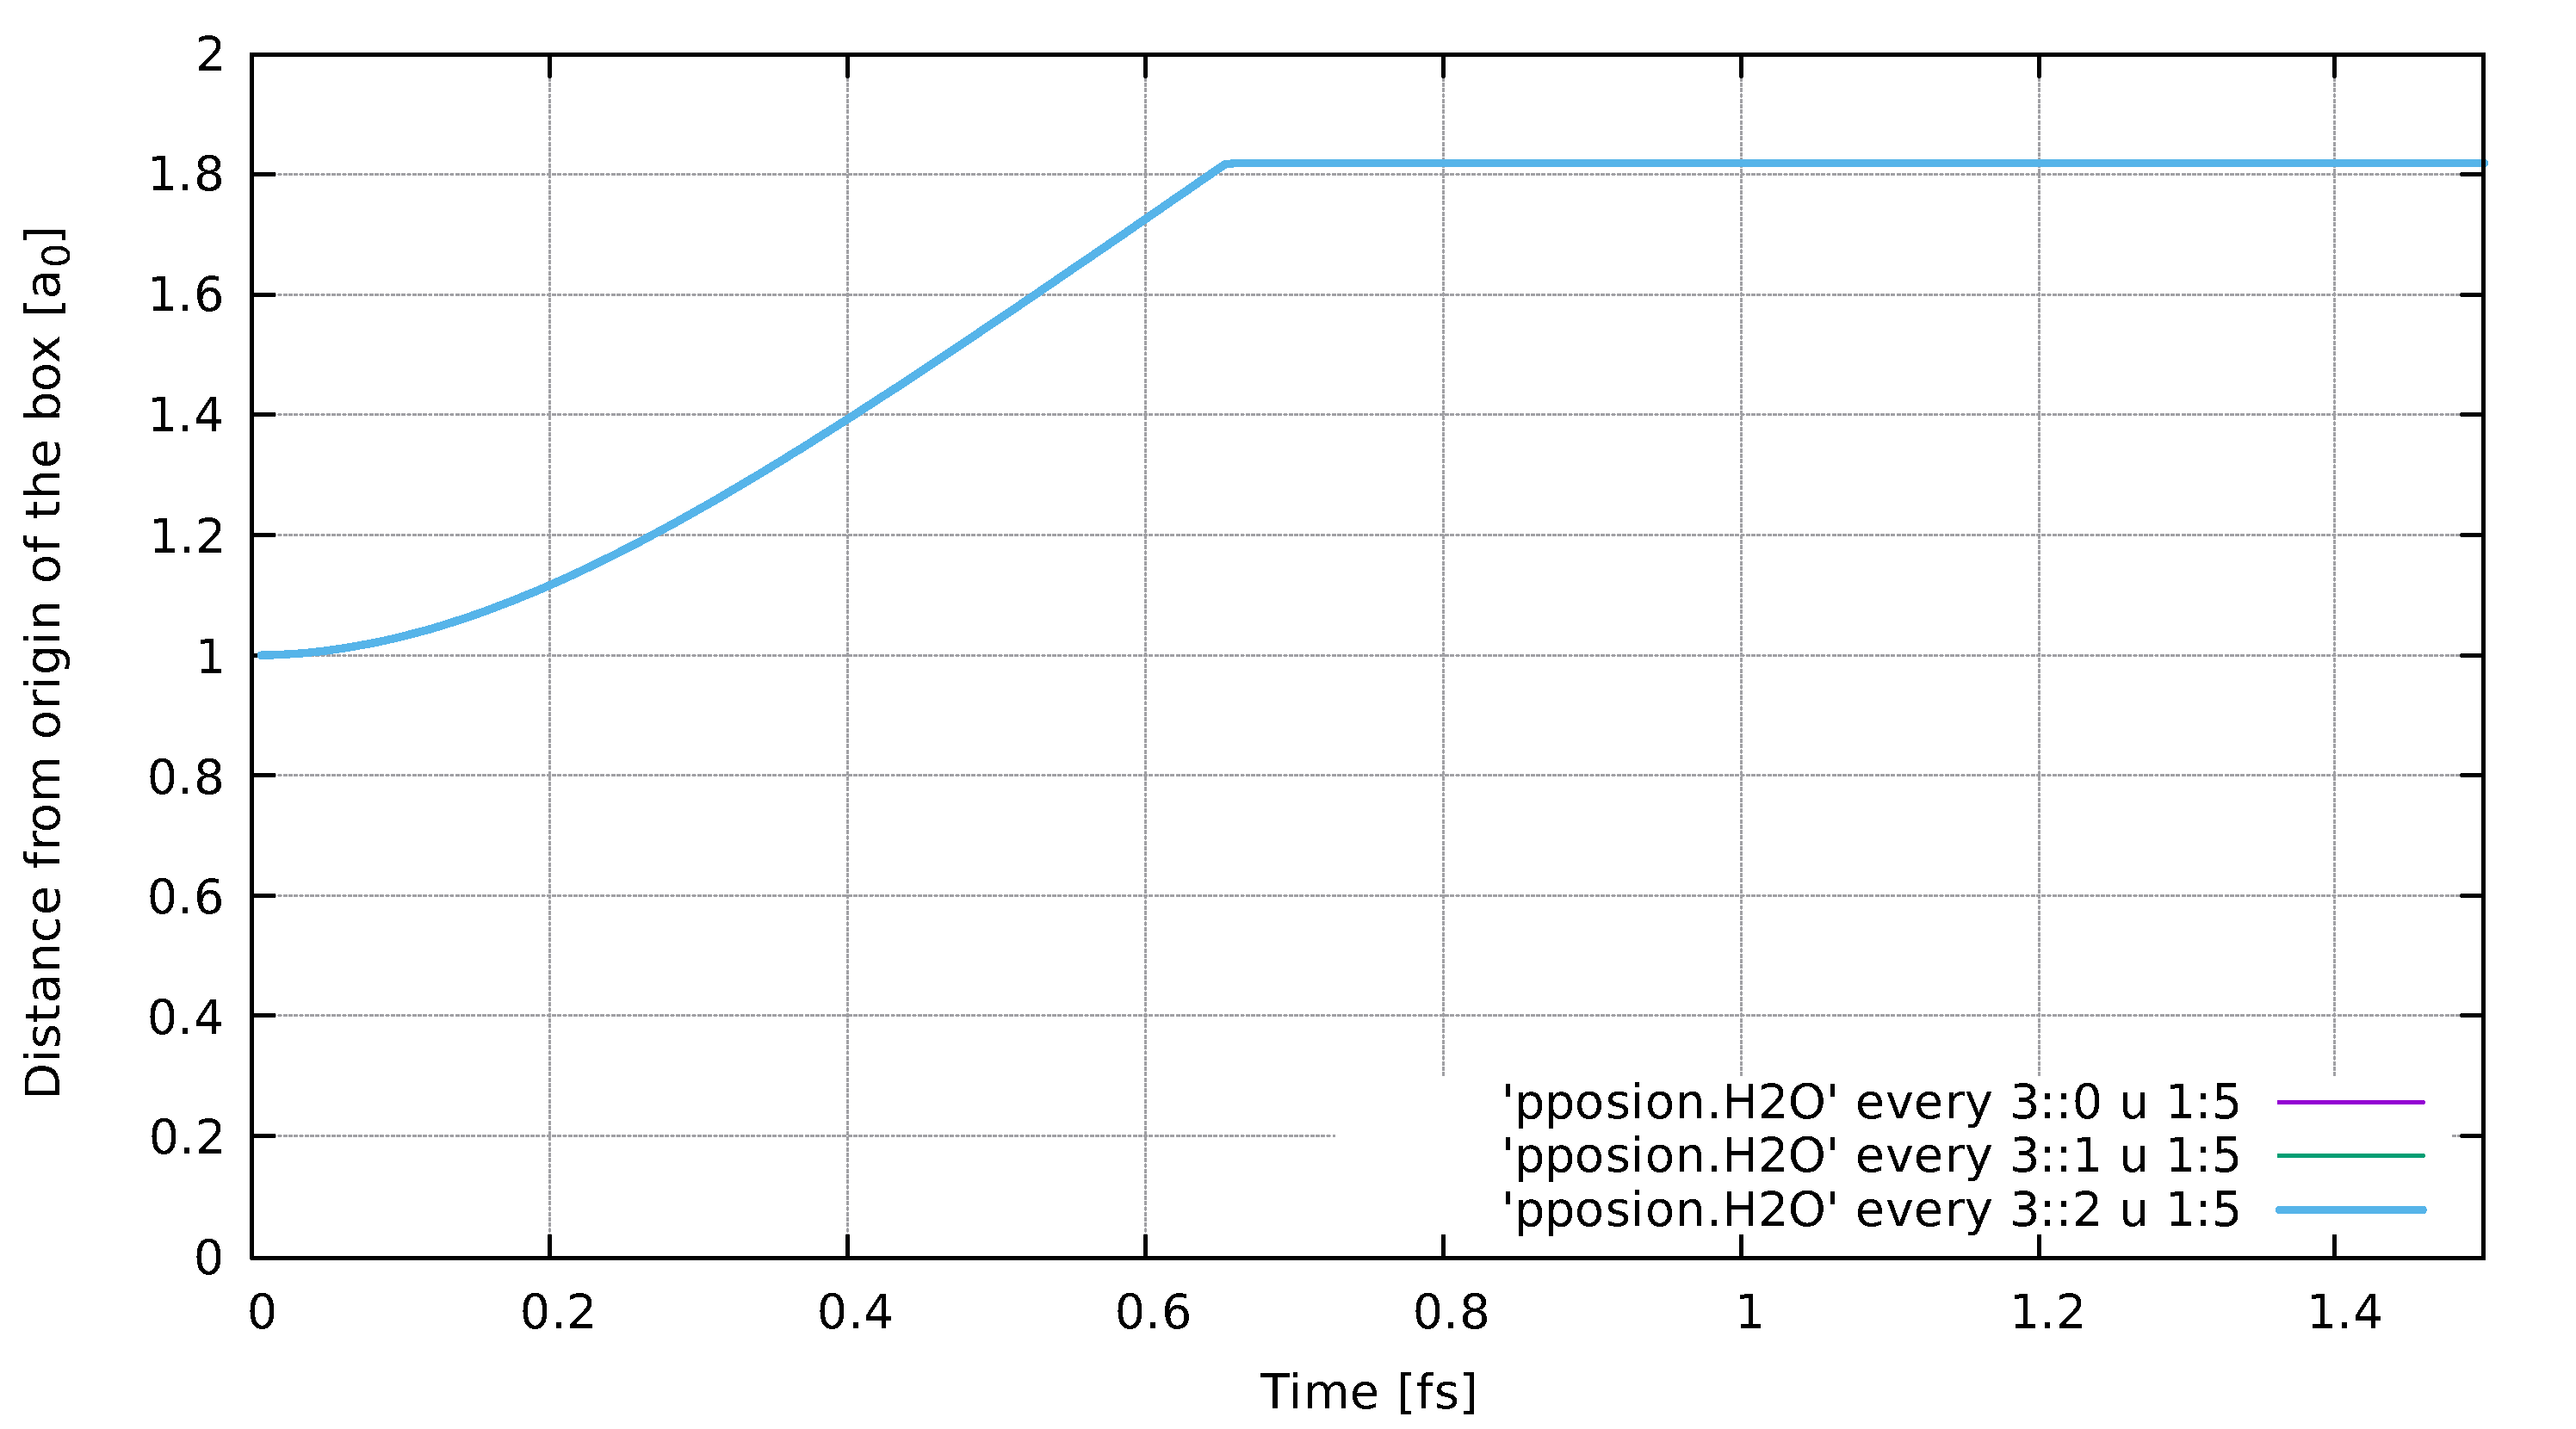
\includegraphics[width=\linewidth]{ionmd_pos}
				\caption{Shows the kinetic energy of the ion cores of oxygen and the two hydrogen atoms respectively as a function of time. After about 0.65~fs the ion cores have reached their equilibrium positions.}\label{fig:ionmd-pos}
			\end{figure}

			\begin{figure}[!htbp]
				\centering
				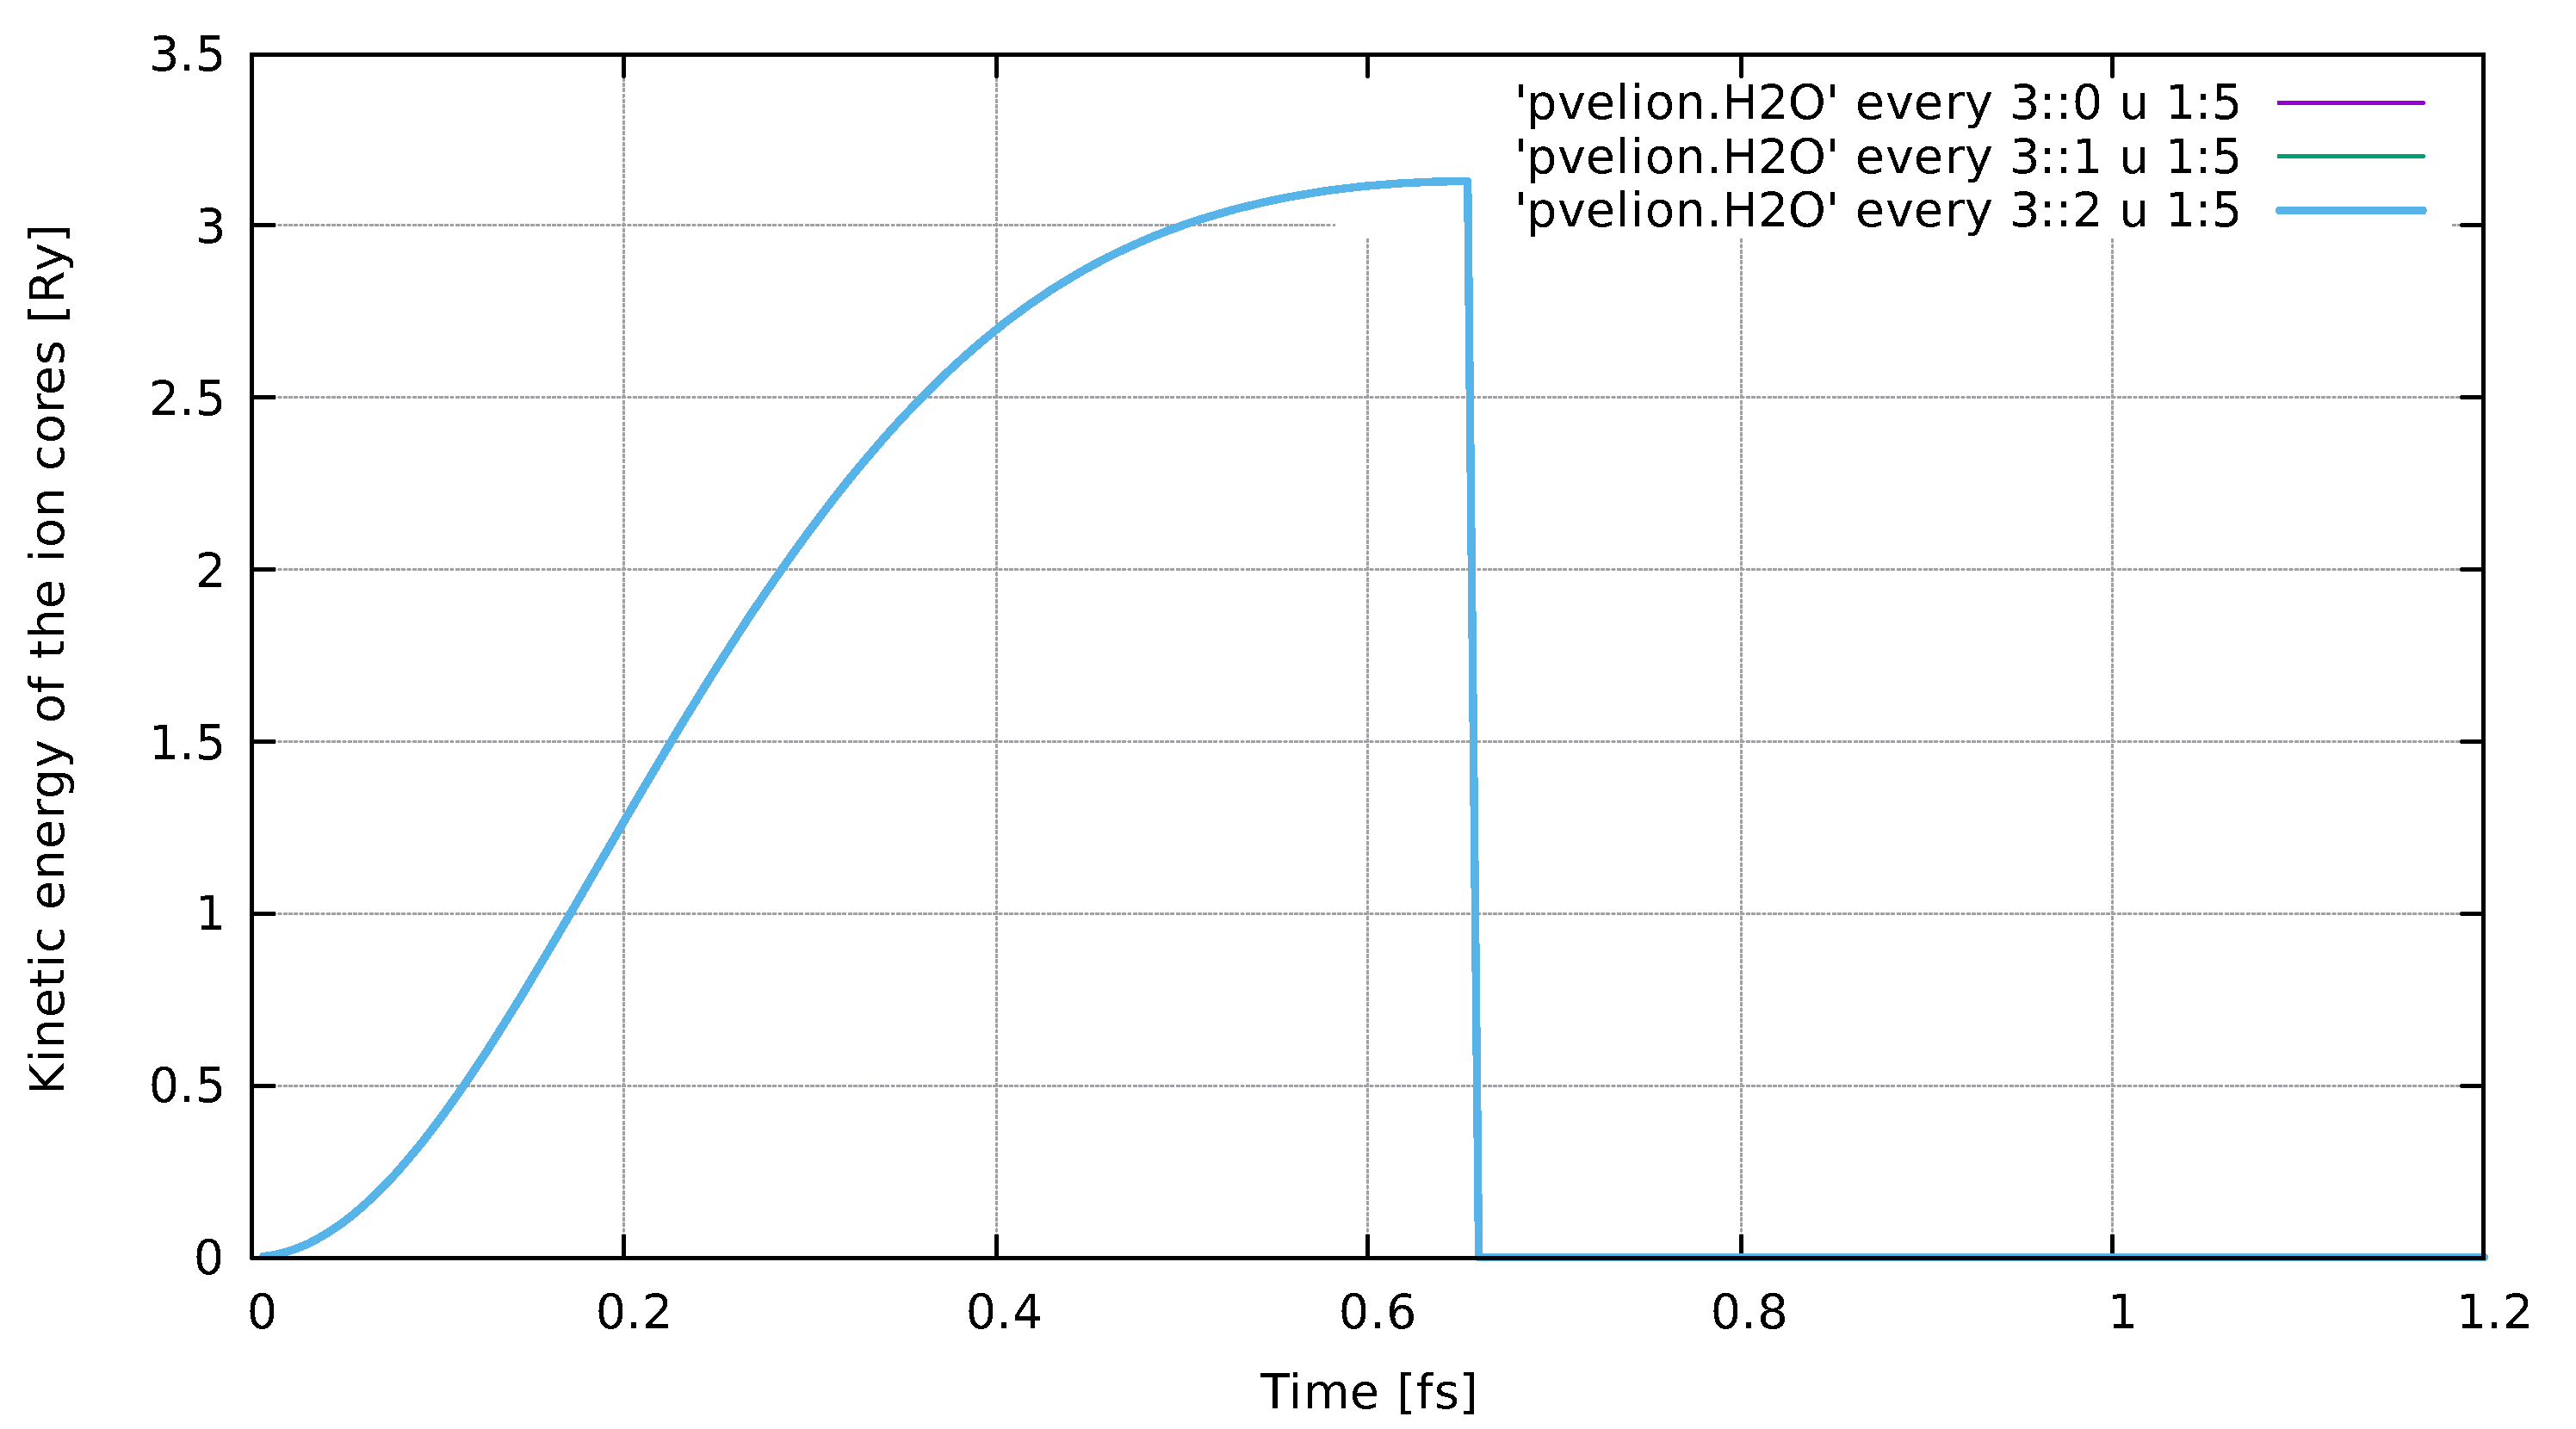
\includegraphics[width=\linewidth]{ionmd_vel}
				\caption{Shows the distance of the ion cores of oxygen and the two hydrogen atoms to the origin of the calculation box as a function of time. After about 0.65~fs the ion cores have reached their equilibrium positions.}\label{fig:ionmd-vel}
			\end{figure}
			
			You can control the interval in number of iterations that the current position and velocity of the ions are printed to these files with \texttt{jpos} and \texttt{jvel}. \figs{fig:ionmd-pos}~and~\ref{fig:ionmd-vel} shows the positions and kinetic energy of the ions during relaxation.
			
			For more detailed information on the dynamic input parameters used here see \tabs{tab:dyn-input-params-general}~and~\ref{tab:dyn-input-params-observables}.

	\section{Basic I/O structure of dynamic calculations}
		In this section the major input parameters will be listed and briefly explained as well as listing of all the generated output files. 
		
		\subsection{Input parameters in the \texttt{DYNAMIC} namelist}
			A list of all the input parameters in the \texttt{DYNAMIC} namelist can be found in \tabs{tab:dyn-input-params-general},~\ref{tab:dyn-input-params-excitation}~and~\ref{tab:dyn-input-params-observables}.
			
			\begin{table}[!htbp]
				\caption{Dynamical paramaters in the DYNAMIC namelist in \texttt{for005.<name>}}\label{tab:dyn-input-params-general}
				\begin{tabular}{|p{3.5cm}|p{11.2cm}|}
					\hline
					\multicolumn{2}{|c|}{The \texttt{DYNAMIC} namelist}\\
					\hline
					\multicolumn{2}{|c|}{\textit{\color{activeColor}numerical and physical parameters for statics and dynamics}} \\
					\hline
					\texttt{dt1}& time step for propagating electronic wave functions,  $\frac{\Delta t}{\Delta x^{2}}\leq 1$\\
					\hline
					\texttt{ismax}& maximum number of static iterations \\
					\hline
					\texttt{idyniter}& switch to s.p. energy as E0DMP for 'iter$>$idyniter'\\
					\hline
					\texttt{ifhamdiag} & diagonalization of m.f. Hamiltonian in static step (presently limited to fully occupied configurations)\\
					\texttt{isitmax}& nr. of imaginary-time steps to improve static solution\\
					\hline
					\texttt{itmax}& number of time steps for electronic propagation\\
					\hline
					\texttt{ifexpevol} & exponential evolution 4. order instead of TV splitting\\
					\hline
					\texttt{iffastpropag} & accelerated time step in TV splitting (for pure electron dynamics, interplay with absorbing b.c. ??)\\
					\hline
					\texttt{irest}& switch to restart dynamics from file 'save'\\
					\hline
					\texttt{istat}& switch to read wavefunctions from file 'rsave'
					\begin{itemize}
						\item it continues static iteration for 'ismax$>$0'
						\item it starts dynamics from these wf's for 'ismax=0'
						\vspace{-3ex}
					\end{itemize}\\
					\hline
					\texttt{idenfunc} & choice of density functional for LDA\\
						& 1 $\rightarrow$ Perdew \& Wang 1992 (default setting)\\
						& 2 $\rightarrow$ Gunnarson \& Lundquist\\
						& 3 $\rightarrow$ only exchange in  LDA \\
					\hline
					\texttt{isave}& saves results after every 'isave' steps \\
					\texttt{}& on file 'rsave' in and after static iteration\\
					\texttt{}& on file 'save' in dynamic propagation\\
					\hline
					\texttt{ipseudo}& switch for using pseudo-densities to represent substrate\\
					\texttt{}& atoms \\
					\hline
					\texttt{ipsptype}& type of pseudopotentials: 0 = soft local (errf);\\
						& 1 = full Goedecker; 2 = local Goedecker;\\
						& 3 = read from file goed.asci (no need to specify)  ;\\
						& 4 = semicore read from file goed.asci\\
					\hline
					\texttt{directenergy}   & \texttt{.true.} = direct computation of energy \\
						& (only for \texttt{LDA}, \texttt{Slater}, \texttt{KLI})\\
					\hline
					\texttt{ifsicp}& selects type of self-interaction correction\\
						&  0 = pure LDA, 1 = SIC-GAM, 2 = ADSIC; 3 = SIC-Slater; \\
						&  4 = SIC-KLI; 5 = exact exchange; 6 = inactive;\\
						&  7 = localized SIC;  8 = full SIC (double set).\\
						& IFSICP=7 or 8 requires switch \texttt{twostsic=1} in \texttt{define.h}.\\
						& Option IFSICP=7 needs yet testing.\\
					\hline
					\texttt{icooltyp}& type of cooling (0=none, 1=pseudo-dynamics,\\
					\texttt{}& 2=steepest descent, 3=Monte Carlo)\\
					\hline
					\texttt{ifredmas}& switch to use reduced mass for ions in dynamics\\
					\hline
					\texttt{ionmdtyp}& ionic propagation (0=none, 1=leap-frog, 2=velocity Verlet)\\
					\hline
					\texttt{ntref}& nr. time step after which absorbing bounds are deactivated\\
					\hline
					\texttt{nabsorb}& number of absorbing points on boundary (0 switches off)\\
					\hline
					\texttt{powabso}& power of absorbing boundary conditions\\
					\hline
					\texttt{ispherabso}& switch to spherical mask in absorbing bounds\\
					\hline
				\end{tabular}
			\end{table}

			\begin{table}[!htbp]
				\caption{Dynamical paramaters in the DYNAMIC namelist in \texttt{for005.<name>}}\label{tab:dyn-input-params-excitation}
				\begin{tabular}{|p{3.5cm}|p{11.2cm}|}
					\hline
					\multicolumn{2}{|c|}{The \texttt{DYNAMIC} namelist}\\
					\hline
					\multicolumn{2}{|c|}{\textit{\color{activeColor}way of excitation}} \\
					\hline
					\texttt{centfx}& initial boost of electronic wavefuncftions in x-direction\\
					\hline
					\texttt{centfy}& initial boost of electronic wavefuncftions in y-direction\\
					\hline
					\texttt{centfz}& initial boost of electronic wavefuncftions in z-direction\\
					\hline
					\texttt{tempion}& initial temperature of cluster ions \\
					\hline
					\texttt{ekmat} & initial kinetic energy of substrate atom (boost in $x$, in eV)\\
					\hline
					\texttt{itft}& choice of shape of laser pulse \\
						&   1 = ramp laser pulse, sine switching on/off\\
						&   2 = gaussian laser pulse \\
						&   3 = cos$^2$ pulse\\
					\hline
					\texttt{tnode}& time (in fs) at which pulse computation starts\\
					\hline
					\texttt{deltat}& length of ramp pulse (\texttt{itft = 1}), in fs\\
					\hline
					\texttt{tpeak}& time (in fs, relative to \texttt{tnode}) at which peak is reached\\
						& (for \texttt{itft} = 1 and 2, pulse length becomes 2*\texttt{tpeak})\\
					\hline
					\texttt{omega}& laser frequency (in Ry)\\
					\hline
					\texttt{e0}& laser field strength in Ry/Bohr\\
					\hline
					\texttt{e1x,e1y,e1z}& orientation of pulse\\
					\hline
					\texttt{e0\_2}& field strength of second laser pulse (only \texttt{itft=3}) \\
					\hline
					\texttt{phase2}& phase of second pulse \\
					\hline
					\texttt{omega2}& frequency of second pulse\\
					\hline
					\texttt{tstart2}& initial ime of second pulse\\
					\hline
					\texttt{tpeak2} & peak time of 2. pulse (pulse length is \texttt{2*tpeak2})\\
					\hline
					\texttt{iexcit} & modus of excitation (0=shifts, 1=rotation)\\
					\hline
					\texttt{iangmo} & switch to compute angular momentum\\
					\hline
					\texttt{irotat} & axis of rotation for excitation (x=1,y=2,z=2,xyz=4)\\
					\hline
					\texttt{phirot} & angle of rotation for excitation (in units of degree)\\
					\hline
					\texttt{phangle} & angle of ``rotation'' into a $1ph$ state\\
					\hline
					\texttt{phphase} & phase of ``rotation'' into a $1ph$ state\\
					\hline
					\texttt{nhstate,npstate}& nr. of hole and particle state for $1ph$ excitation\\
						& this $1ph$ option can only be run from \texttt{istat=1}\\
					\hline
					\texttt{eproj}& energy of incoming projectile (= last ion in the list)\\
					\hline
					\texttt{vpx,vpy,vpz}& direction of the incoming projectile\\
					\hline
					\texttt{taccel}& time span over which the projectile is accelerated to \texttt{eproj}\\
						& for \texttt{taccel=0} one has to use \texttt{init\_lcao=1}\\
					\hline
				\end{tabular}
			\end{table}


			\begin{table}[!htbp]
				\caption{Parameters that control observables and output in the DYNAMIC namelist in \texttt{for005.<name>}}\label{tab:dyn-input-params-observables}
				\begin{tabular}{|p{3.5cm}|p{11.2cm}|}
					\hline
					\multicolumn{2}{|c|}{The \texttt{DYNAMIC} namelist}\\
					\hline
					\multicolumn{2}{|c|}{\textit{\color{activeColor}flags for observables}} \\
					\hline			
					\texttt{iemomsRel}& calculates multipole momentas of electron density relative to origin (0) or c.m. of cluster (1)\\
					\hline
					\texttt{istinf}& modulus for printing information in static iteration \\
					\hline
					\texttt{ifspemoms}& switch to compute and print spatial s.p. moments\\
					\hline
					\texttt{iftransme}& switch to compute and print transition m.elements\\
					\hline
					\texttt{ifrhoint\_time}& switch to slices of integrated densities for all times\\
					\hline
					\texttt{jstinf}& modulus for printing information in dynamic \\
					\hline
					\texttt{jinfo}& modulus for printing dynamical information on \texttt{infosp.<name>} \\
					\hline
					\texttt{jdip}& modulus for printing dipole moments on \texttt{pdip.<name>}\\
					\hline
					\texttt{jquad}& modulus for printing quadrupole moments on \texttt{pquad.<name>}\\
					\hline
					\texttt{jesc}& modulus for printing ionization \texttt{pescel.<name>}\\
					\hline
					\texttt{jenergy}& modulus for printing energy information on \texttt{penergies.<name>} \\
					\hline
					\texttt{iflocaliz}& activates computation of Becke's localisation\\
					\hline
					\texttt{jelf}& modulus for analysing and printing electron localisation in dynamics various files are written of the form \texttt{pelf*.<name>}\\
					\hline
					\texttt{iflocaliz}& modulus for analysing and printing electron localisation in statics\\
					\hline
					\texttt{jstinf}& modulus for printing s.p. energies and variances\\
					\hline
					\texttt{jpos}& modulus for printing ionic positions on \texttt{pposion.<name>}\\
					\hline
					\texttt{jvel}& modulus for printing ionic velocities on \texttt{pvelion.<name>}\\
					\hline
					\texttt{jstateoverlap}& switch to compute overlap of static state with the state directly after dynamical initialisation\\
					\hline
				\end{tabular}
			\end{table}

		\subsection{Output files}
		
			A list of all the output files and their description can be found in \tabs{tab:dynamic-output-files}~and~\ref{tab:dynamic-output-files-cont}.
			
			\begin{table}[!htbp]
				\caption{Output files generated during a dynamic calculation}\label{tab:dynamic-output-files}
				\begin{tabular}{|p{4.5cm}|p{10.2cm}|}
					\hline
					\texttt{energies.<name>} & historical, contains only the binding energy\\
					\hline
					\texttt{forces.<name>} & forces on ions, generated when ion molecular dynamics is active\\
					\hline
					\texttt{<name>.bs} & output suited for further processing by freeware which  can make 3D structure plots of molecular configurations in the typical chemical style\\
					\hline
					\texttt{pdip.<name>} &  dipole moment in x, y, z direction, versus time \\
					\hline
					\texttt{penerclu.<name>} & kinetic energy of the cluster in the x,y,z directions and total, versus time, at intervals commanded by the input parameter jener\\
					\hline
					\texttt{pescel.<name>} & proportion of electrons remaining, total number of electrons, number of electrons lost, versus time, at intervals commanded by the input parameter jesc\\
					\hline
					\texttt{plaser.<name>} & laser parameters Ex, Ey, Ez, power, laser energy, etc as a fonction of time\\
					\hline
					\texttt{povlp.<name>} & unused in this version\\
					\hline
					\texttt{penergies.<name>} & Various energies, versus time. The 26 detailed entries (single particle energy, rearrangement energy, etc..) are described in the output file itself. The total energy is at location 18. \\
					\hline
					\texttt{pescOrb.<name>} & Number of electrons lost per orbital, versus time, at intervals commanded by the input parameter jnorms \\
					\hline
					\texttt{pkinenion.<name>} & kinetic energy of the cluster in the x,y,z directions and total, versus time, at intervals commanded by the input parameter jpos\\
					\hline
					\texttt{pPES.<name>} & unused in this version\\
					\hline
				\end{tabular}
			\end{table}

			\begin{table}[!htbp]
				\caption{Output files generated during a dynamic calculation (\emph{continued})}\label{tab:dynamic-output-files-cont}
				\begin{tabular}{|p{4.5cm}|p{10.2cm}|}
					\hline
					\texttt{pposion.<name>} & positions of the individual ions in x,y,z, and distance to center, versus time, at intervals commanded by the input parameter jpos\\
					\hline
					\texttt{pproba.<name>} & probabilities of charge states versus time, at time intervals commanded by input parameter jnorms\\
					\hline
					\texttt{pprojdip.<name>} & x, y, z pos of projectile versus time, at time intervals commanded by input parameter jdip\\
					\hline
					\texttt{prhov.<name>} & unused in this version\\
					\hline
					\texttt{progstatus} & Only a flag when dynamics are finished\\
					\hline
					\texttt{pspenergies.<name>} & single particle energies versus time, at time intervals commanded by input parameter jinfo\\
					\hline
					\texttt{pspvariances.<name>} & single particle energy variances versus time, at time intervals commanded by input parameter jinfo\\
					\hline
					\texttt{pspvariancesp.<name>} & single particle energy variances versus time (with correction by projection), at time intervals commanded by input parameter jinfo \\
					\hline
					\texttt{ptempion.<name>} & ion temperatures during ionic-core relaxation\\
					\hline
					\texttt{pvelion.<name>} & ion velocities during ionic-core relaxation, or dynamic calculation with molecular dynamics\\
					\hline
					\texttt{rsave.<name>} & This file contains all parameters of a static convergence to allow for a dynamic start without recomputing the statics: to use it set ismax=0 and istat=1  \\
					\hline
					\texttt{save.<name>} & This file contains all parameters to allow for a dynamic start at time : to use it set  irest>=0 \\
					\hline
					\texttt{Time} & Number of points in the calculation box and used wall time to complete the given number of iterations\\
					\hline
				\end{tabular}
			\end{table}

	\section{An example dynamic calculation for H$_\mathsf{2}$O}

		\subsection{Excitation by applying a LASER pulse}
			In this example we will excite the water molecule by applying a resonant and off-resonant LASER pulse. The example input files can be found in
			\begin{verbatim}
				$QDD_ROOT/examples/H2O/dynamic/
			\end{verbatim}
			The most important parameters that control the laser excitation are the following		
			\begin{verbatim}
				itft = 3
				deltat = 36.0
				e1x = 0.0
				e1y = 0.0
				e1z = 1.0
				omega = 0.79
				e0 = 0.08
			\end{verbatim}
			The be on-resonance we need an \texttt{omega} of 0.79~Ry which corresponds to 10.7~eV. In this case the pulse shape is a $\cos^2$, the pulse length is 36~fs and the pulse polarisation is in the $z$-direction. A list of all the excitation parameters can be found in \tab{tab:dyn-input-params-excitation}.
			
			To calculate the off-resonant case, simply change the value of \texttt{omega} to another value, e.g. 0.691~Ry, or 9.4~eV.
		
		\subsection{Results and observables}	
			Three basic observables, the ionisation, absorption and dipole moment are shown in \figs{fig:h2o-onres}~and~\ref{fig:h2o-offres} (the green curves). \fig{fig:h2o-onres} shows the time evolution of the three key observables considered in the present study. The dipole signal (lower panel) starts like an off resonant response where laser pulse and dipole signal follow the same pattern. At about 15~fs, we see a sudden increase in response and the dipole signal quickly deviates from the laser pulse, a typical pattern of resonant excitation.
	
	\section{Electronic relaxation with RTA}
	
		\subsection{Additional \texttt{DYNAMIC} input parameters concerning RTA}
			One can simply use the input files from the previous section at
			\begin{verbatim}
				$QDD_ROOT/example/H2O/dynamic/
			\end{verbatim}
			 and enable the RTA procedure by choosing an iteration interval for an RTA step to happen. If want an RTA-step to happen every 1000 iteration set
			\begin{verbatim}
				jrtaint = 1000
			\end{verbatim}
			A list of all the input parameters in the \texttt{DYNAMIC} namelist related to RTA can be found in \tab{tab:dyn-input-params-rta}.

			\begin{table}[!htbp]
				\caption{Parameters that control RTA in the DYNAMIC namelist in \texttt{for005.<name>}}\label{tab:dyn-input-params-rta}
				\begin{tabular}{|p{3.5cm}|p{11.2cm}|}
					\hline
					\multicolumn{2}{|c|}{The \texttt{DYNAMIC} namelist}\\
					\hline
					\multicolumn{2}{|c|}{\textit{\color{activeColor}flags for RTA}} \\
					\hline			
					\texttt{jrtaint} &  Modulus for calling the RTA subroutine, i.e., nr. of TDLDA steps per one RTA step. Course time step $\Delta t$ for RTA and fine time step for TDLDA \texttt{dt1} are related as $\Delta t=$\texttt{jrtaint}$*$\texttt{dt1}.\\
					\hline
					\texttt{rtamu} & Parameter $\mu$ in front of the quadratic density constraint in the DCMF Hamiltonian (\ref{eq:hDCMF})\\
					\hline
					\texttt{rtamuj} & Parameter $\mu_j$ in front of the quadratic current constraint in the DCMF Hamiltonian (\ref{eq:hDCMF})\\
					\hline
					\texttt{rtasumvar2max} & Termination criterion $\epsilon_0$ in the RTA step as used in figure \ref{fig:summaryDCMF}\\
					\hline
					\texttt{rtaeps} & Step size $\delta$ in the damping operator (cross ref to be defined) $\mathcal{D}$ for the RTA step.\\
					\hline
					\texttt{rtae0dmp} & Energy offset $E_{00}$ in the damping operator (cross ref to be defined) $\mathcal{D}$ for the RTA step\\
					\hline
					\texttt{rtasigee} & In medium $e^--e^-$ cross section used for the relaxation time (\ref{eq:relaxtime})\\
					\hline
					\texttt{rtars} & Effective Wigner-Seitz radius $r_s$ used for the relaxation time (\ref{eq:relaxtime})\\
					\hline
					\texttt{rtatempinit} & The value \texttt{rtatempinit}/10 is used as lower value for the search of temperature in \texttt{SUBROUTINE ferm1}\\
					\hline
				\end{tabular}
			\end{table}

		\subsection{Output files}
			A list of all the output files and their description can be found in \tab{tab:dynamic-output-files-rta}.
			
			\begin{table}[!htbp]
				\caption{Output files that are specific to a RTA-enabled calculation}\label{tab:dynamic-output-files-rta}
				\begin{tabular}{|p{4.5cm}|p{10.2cm}|}
					\hline
					\texttt{convergenceRTA} & this file contains a log of the RTA iterations that contains information on the convergence details\\
					\hline
					\texttt{peqstate} &  parameters for convergence of the dtmf process: current iteration number, cycles to convergence, variance, residual err. on density, residual err. on current, parameters mu, muj, energy achieved\\
					\hline
					\texttt{prta} & prints at each RTA  step: time, entropy, laser energy and the mu and temperature of a fermi distribution fitted to the occupation numbers\\
					\hline
					\texttt{pspeed.<name>} & prints at each RTA step, along x axis, the reference density (spin up and down), achieved density (spin up and down), target x current, achieved x current \\
					\hline
				\end{tabular}
			\end{table}
			
		\subsection{The effect of dissipation on resonant and off-resonant excitation of H$_\mathsf{2}$O}
			Of particular interest is the performance of RTA as compared to LDA. In \fig{fig:h2o-onres} for the first 15~fs there is practically no difference between LDA and RTA. Dissipation depends strongly on internal excitation energy and is thus inactive in the early stages, where not yet enough energy has been absorbed (middle panel). Later on, the difference grows dramatic. Dipole oscillations last very long after the pulse in the case of LDA, while RTA produces considerable attenuation.
			
			Dissipation produces also a different evolution of energy absorption (middle panel) to the extent that more energy can flow into the system. The mechanism is a suppression of induced emission. If a system undergoes dipole oscillations in resonance with the laser field photon emission is coherently amplified and at a certain stage more energy is emitted than absorbed. This is the mechanism known as Rabi oscillations in simple two-level systems, and it leads to the observed oscillations in $E_\mathrm{abs}$. Unlike in two-level systems, the photon couples here to several dipole modes which reduces the amplitude of the Rabi oscillations. Dissipation, furthermore, transfers energy out of the resonant dipole channel into intrinsic excitation as seen from the then smaller dipole amplitude (lower panel). This reduces induced emission and thus gives the system new capacity to swallow more energy. It is a question of subtle energy balance in the system how this surplus on energy is distributed.
			
			The upper panel of \fig{fig:h2o-onres} shows the time evolution of ionisation. Dissipation in RTA distracts electrons from their way to direct emission and redirects them to the system enhancing its intrinsic energy. Thus ionisation is with RTA systematically lower than with LDA. Another difference is seen in the long-time behaviour. In RTA, ionisation levels off after the pulse is over while it carries on in LDA. The latter is related to the long lasting dipole oscillations which continue to feed the emission channel.
			
			\fig{fig:h2o-offres} shows time evolution for off-resonant excitation of H$_2$O. In fact, we see that the case shows traces of resonance response in the very early stages. But later on, the dipole signal (lower panel) follows in the average the pulse envelope and, most important, it nearly disappears with the pulse dying out. Being not perfectly off-resonant, the system’s modes remain somewhat excited as one can see from energy absorption (middle panel) not fully returning to zero. It is much smaller than in the resonant case, but it is not returning fully back to zero which indicates some energy transfer away from the coherent dipole oscillations into other systems modes. The energy thus absorbed is distributed into continuum modes which leads to direct ionisation (see upper panel) and into bound modes which leaves eventually some final intrinsic excitation.
			
			\begin{figure}[!htbp]
				\centering
				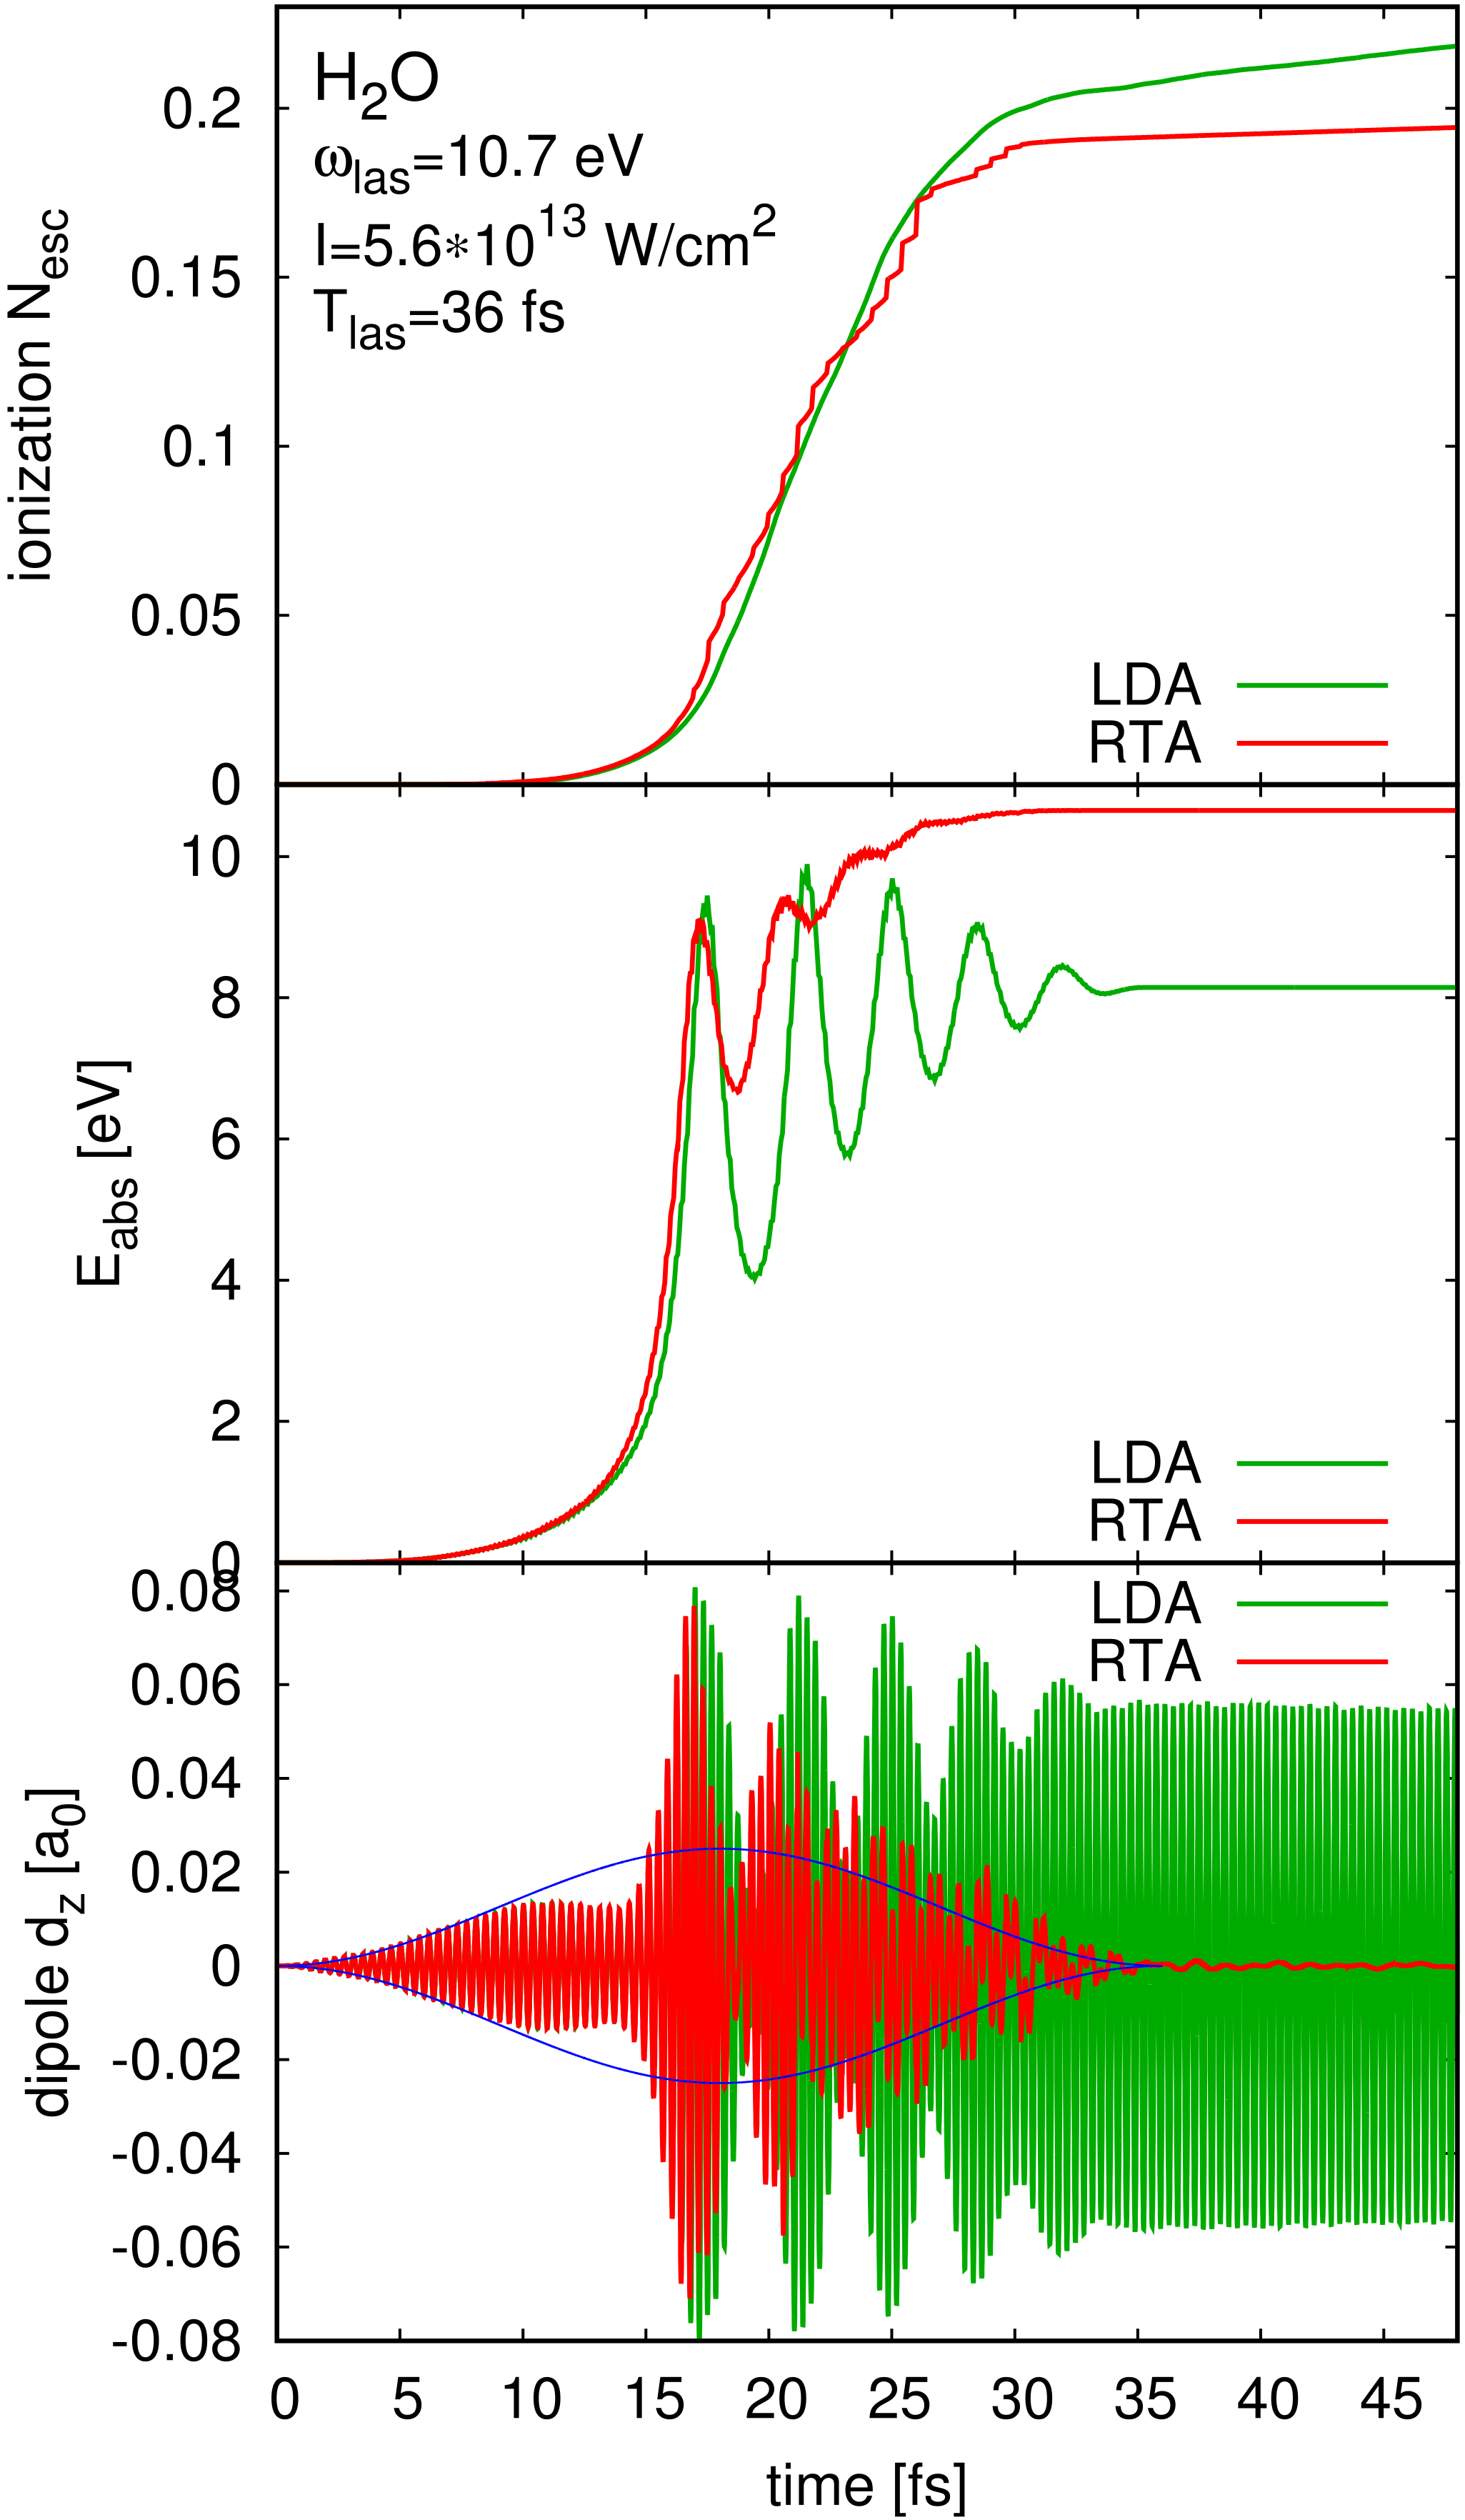
\includegraphics[width=0.75\linewidth]{h2o-onres}
				\caption{Comparison of LDA and RTA time evolution of three basic observables for H$_2$O: dipole moment perpendicular to molecular plane (lower), energy absorbed from laser field (middle), and net ionisation (upper). In the lower panel, the pulse envelope is indicated in addition to the dipole moments. The system was excited by a laser pulse with frequency $\omega_\mathrm{las}=10.7$~eV, intensity $I=5.6\times10^{13}$~W/cm$^2$, and total pulse length $T_\mathrm{pulse}=36$~fs.\\{\sffamily\itshape Image from Phys.~Plasmas~\textbf{25},~031905~(2018).}}\label{fig:h2o-onres}
			\end{figure}

			\begin{figure}[!htbp]
				\centering
				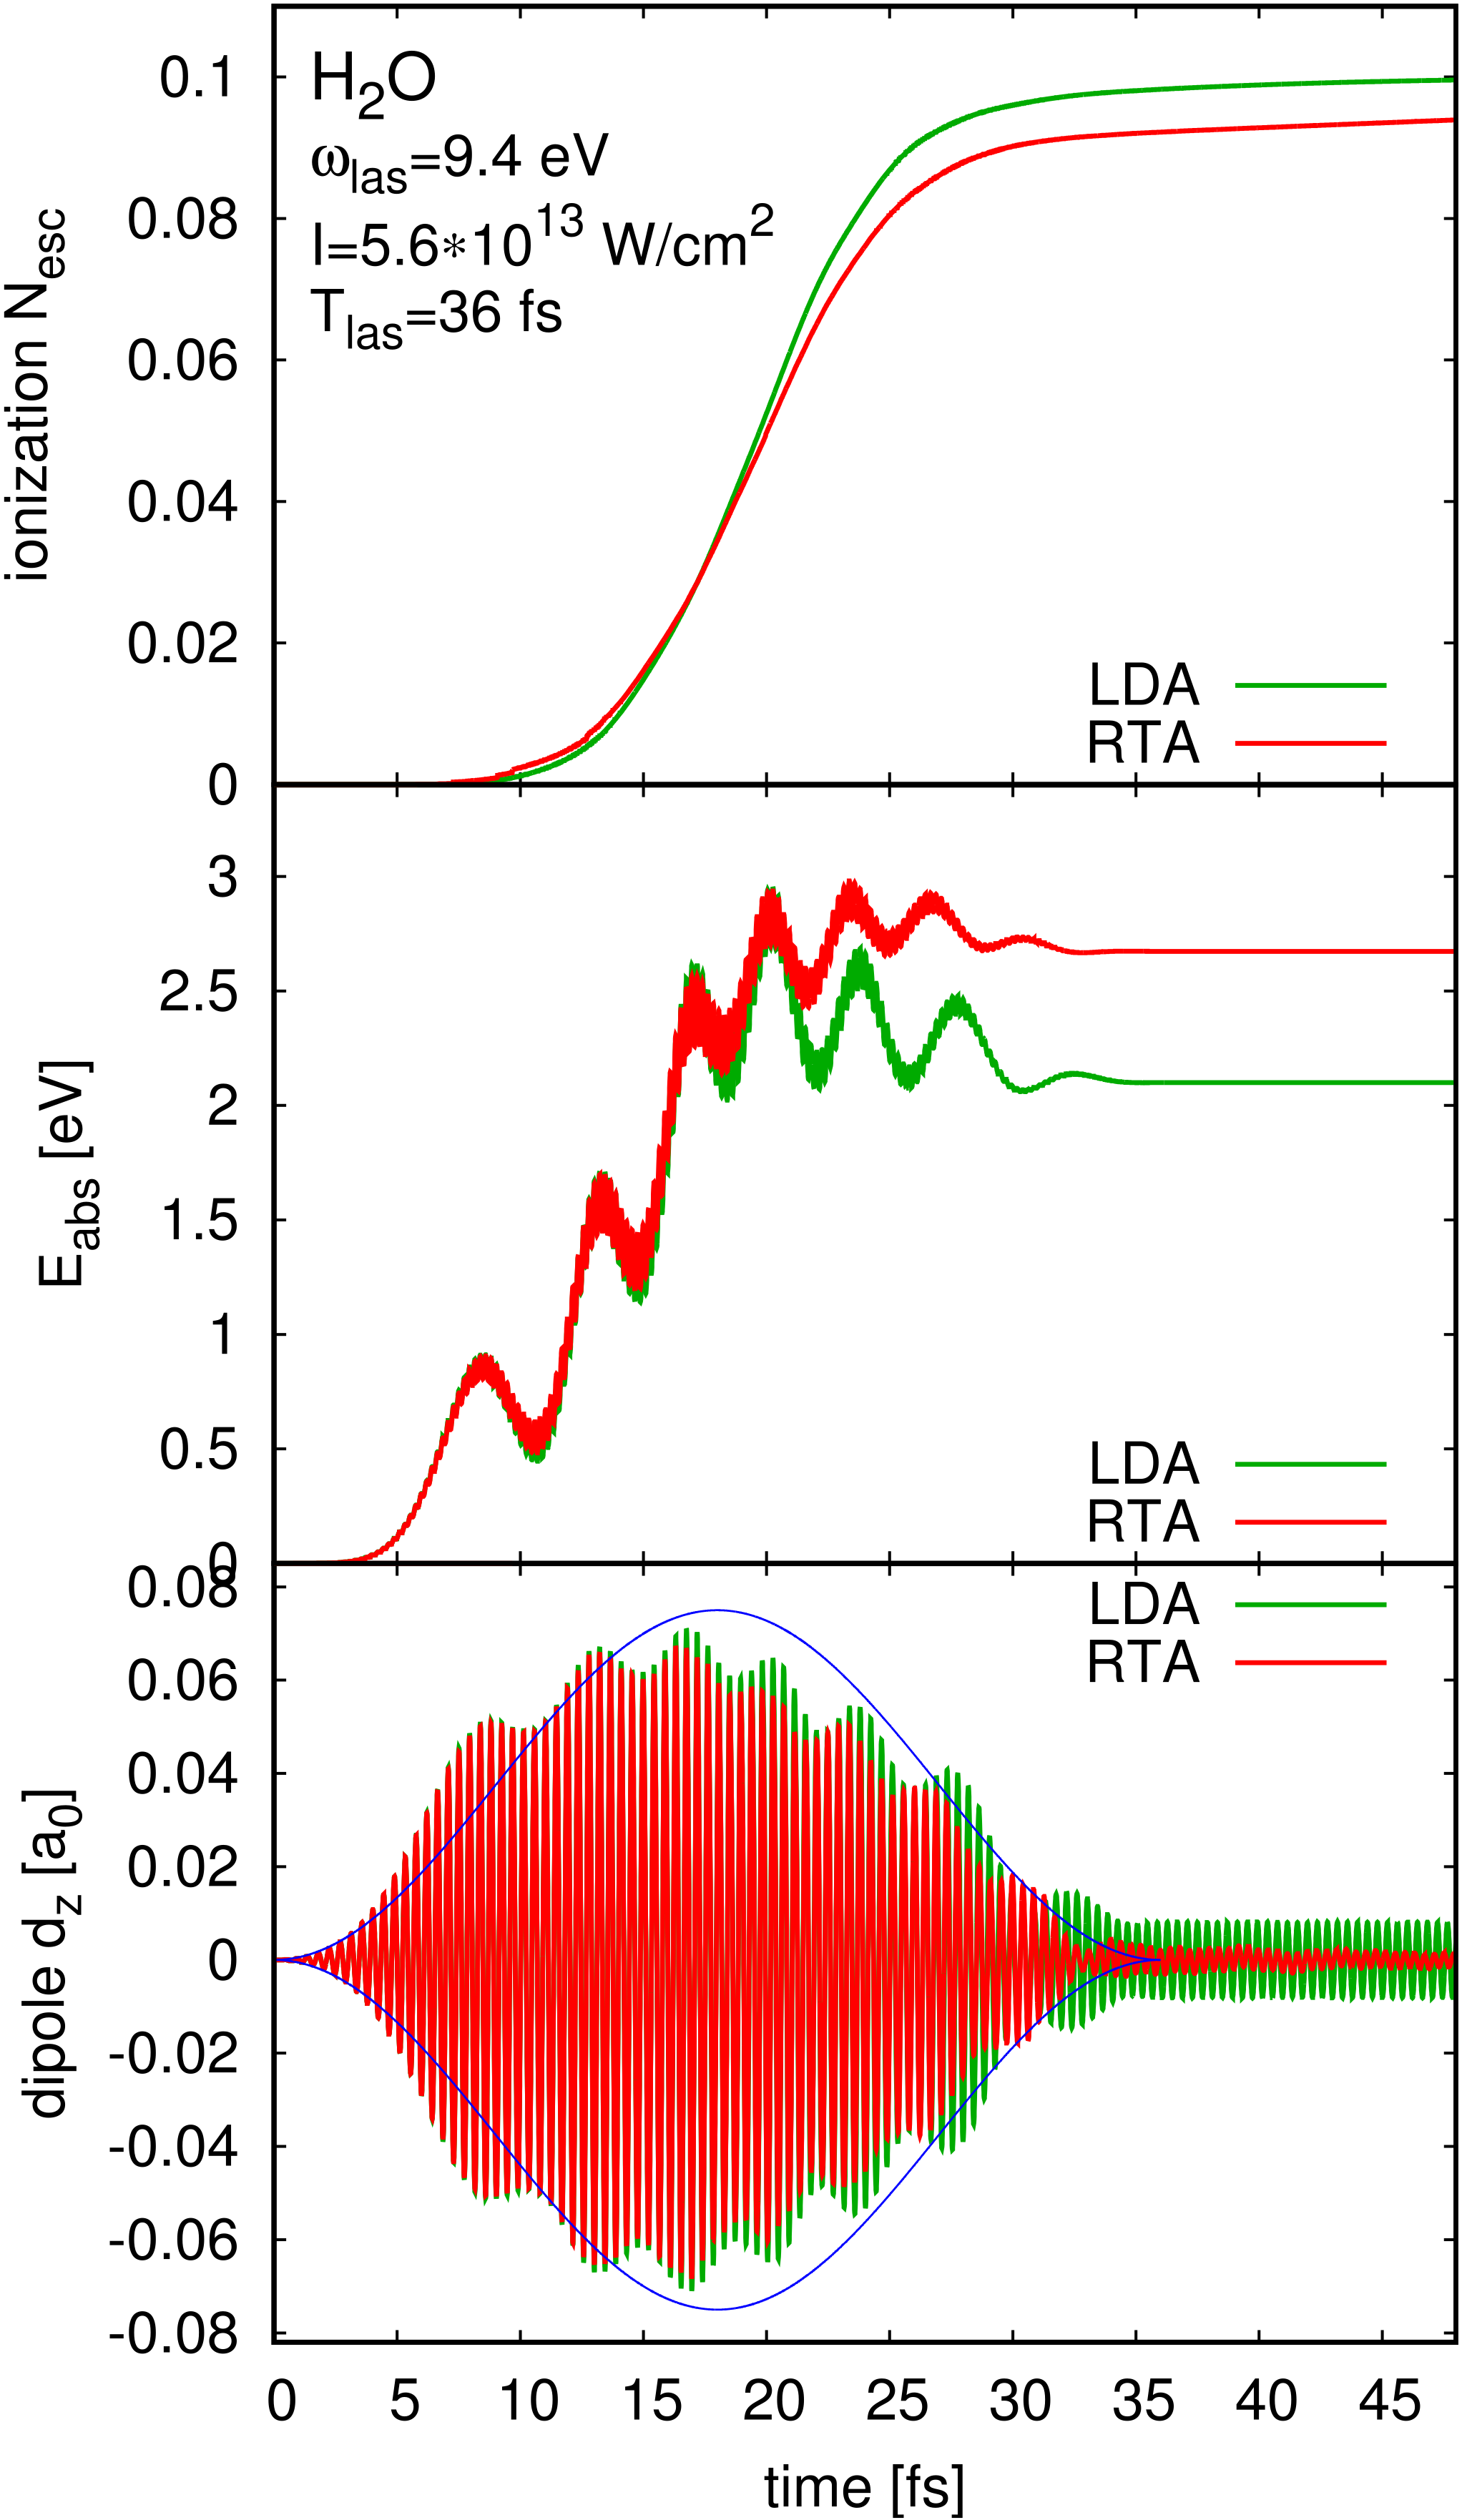
\includegraphics[width=0.75\linewidth]{h2o-offres}
				\caption{Same as \fig{fig:h2o-onres} but off-resonance at $\omega_\mathrm{las}=9.4$~eV. \\{\sffamily\itshape Image from Phys.~Plasmas~\textbf{25},~031905~(2018).}}\label{fig:h2o-offres}
			\end{figure}
			
			
			
								
%	\section{General thoughts and suggestions}
%	Some interesting test cases could be
%	\begin{itemize}
%		\item H$_2$O: Non-trivial molecule
%		\item Na$_7$: this is an interesting case because instead of preferring to be in a tetrahedral configuration, it prefers to be in a planer configuration.
%		\item Na$_{12}$: this is the first spin-polarised (has to be checked) cluster consisting of an even number of electrons.
%		\item The carbon chains C$_3$, C$_5$ and C$_7$: they all exhibit both organic- and metallic properties and have well defined plasmon modes. Furthermore, since these are all 1D and planar molecules, they can be calculated in a 1D or 2D box which makes the calculation much faster.
%		\item Na$_{93}$, : This is a magic number too.
%	\end{itemize}
	\end{document}